%-------------------------------------------------------------------------------
\section{Motivation}\label{motivation}
%-------------------------------------------------------------------------------

This paper is motivated by the benefits of serverless as an approach to utility
computing, and finds latency variability to be a key challege in making true
serverless a reality.

\subsection{Benefits of serverless}

The main attraction of serverless for developers is, in an idealized world, the
characteristic of paying only for what they use, while having a whole datacenter
available to them. This proposition is especially attractive to developers of
applications where the amount of resources that they need varies significantly
over time, or is generally small and very spread out. With such workloads,
buying their own machines or renting a fixed amount of server space is bad for
the developer because it is expensive if provisioned for peak usage and has poor
performance if not, and bad for providers because it leads to low utilization.

A central example to this paper is that of a web server. Its traffic patterns
make it a great candidate for running as serverless functions: it is
event-based, its load is bursty and unpredictable, and a request's resource
requirements can vary greatly depending on which user invoked it.


A back of the envelope calculation shows that for web servers with small load,
lambda functions as they stand today are cheaper: for a low-traffic website,
with approx 50K requests per day, a memory footprint of < 128 MB, and 200ms of
execution, running that on AWS lambda adds up to \$1.58 per month. On the other
hand, the cheapest EC2 instance costs just over \$3 per month. Of course, as the
number of requests goes up, the price for lambdas scales linearly, whereas
running an EC2 instance on full load becomes comparably cheap. Extensive
simulations show a more nuanced picture of the tradeoff points for different
workloads~\cite{econ-of-serverless,trek10-blog}.

Serverless also may outperform reservation systems for workloads that are very
bursty: starting a new lambda execution environment is much faster than starting
a new container or EC2 instance, which can take multiple
minutes~\cite{ec2-autoscaling}.


\subsection{Challenge of latency variability}


\begin{figure}[t!]
    \centering
      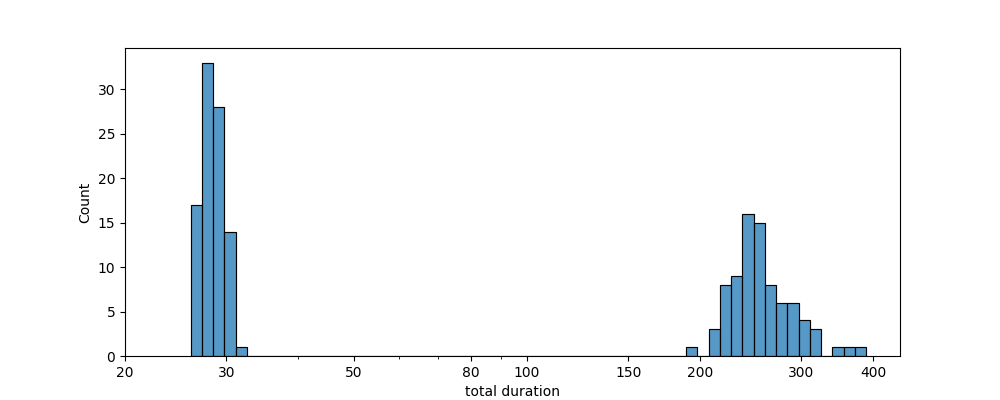
\includegraphics[width=8.5cm]{img/lambda_total_durations.png}
      \caption{ distribution of end to end duration times. The y axis is log scale }
    \label{fig:lambda-total-durations}
\end{figure}

However, only few web applications run entirely on serverless offerings today.
There are many reasons that developers choose not to use serverless, despite
their workloads being well-suited for the serverless
environment~\cite{not-lambda-blog,reddit-serverless2}. Popular complaints
include provider lock in, lack of insight for debugging and telemetry, and
variable runtimes.


\Sys{} focuses on the challenge of variable runtimes. In order to better
understand the where the variation comes from, we run an experiment with a
simple lambda function that sleeps for 20ms and then returns. We use AWS
Xray~\cite{aws-xray} to measure its latency, with incovations spaced randomly
between 0 and 10 minutes. The results are in
Figure~\ref{fig:lambda-total-durations}. The spike on the left side of the graph
is the execution times from invocations that used warm start. We can see the
durations remain stable. The reason for this is that AWS is able to simply route
the new request to the machine with the existing container on it. We verify that
this is indeed what is happening by changing the function to include reading and
then writing to an environment variable, and find that for invocations with warm
start when we read the variable it was already set by a previous invocation.


The right grouping in the graph is those invocations that hit cold starts, whose
overall latencies vary between $\sim$200 and $\sim$400ms.


In order to understand where the extra latency in the longer times comes from,
we begin by ruling out some options such as container downloading, and then look
to open source alternatives to come to the conclusion that it comes from
queueing or delay (waiting for resources) in the system.

???

\hmng{What we are trying to show here is that the stable latencies from warm
start wouldn't spill over into the cold start world even if cold start is fast? Or
maybe a flipside of that which is that part of the cold start latency comes from
queuing already now? Those feel like two different things --- one is more the
breakdown thing, the other is more the openwhisk experiment with everything warm
start}


Indeed, it must be the case that any system that runs with high average
utilization experiences moments where there is more load than the resources can
handle. As we know from recent traces~\cite{prequal}, although load may look
stable at a time increment of hours or even minutes, going down to the second
and millisecond level shows the load to have high variance. If providers want to
have good average utilization, then in the moments of load spike the load will
be more than the resources can handle.

The scheduler then has two different options: queue the excess load, or place it
on machines and let them deal with being temporarily overloaded. Different
schedulers have different approaches. In OpenWhisk~\cite{openwhisk}, for
instance, the load balancer will choose which machine to run the function on,
and then place the invocation, adressed to that machine, into a Kafka queue that
the machine subscribes to and can pull the invocation from when it is
ready~\cite{openwhisk-sched}. Knative~\cite{knative} similarly queues the excess
invocations, although it does so via the load balancer, which is also in charge
of autoscaling~\cite{knative-sched}: if the existing pods are fully loaded (with
a small, bounded-size queue in front of them), requests are queued separately
while the autoscaler starts up more invocations. It is impossible to know what
proprietary systems like AWS do, but since AWS guarantees an amount of memory as
well as a fraction of vCPUs to each function, it is likely AWS also queues the
invocations to ensure they aren't put in a position of having to break those
guarantees.\hmng{that might be a test we could run: do a tight while loop and
look at cpu time and wall clock time to see how we are being scheduled}

Because none of these schedulers have information about the functions they are
queueing, it is impossible for them to know which to prioritize. Without further
tooling, it is possible and in fact likely that latency sensitive jobs might end
up in the queue behind background functions. The way all of the above schedulers
deal with this is by doing some sort of accounting of concurrency: concurrency
can be reserved or provisioned for specific functions, and limited for others.
This is necessary to ensure that a burst in background tasks doesn't starve the
latency sensitive functions. However, what happens when the datacenter is out of
resources and so the concurrency limit has not yet been reached but the
resources are unavailable is not clear. Reserving and provisioning and limiting
are also conceptually in tension with the goal of serverless, which is to be
on-demand and flexible.









